%!TEX root = ../Touch Based Idris.tex 
\chapter{Architecture}
\label{sec:Architecture}

We decided to write our app for the Apple iPad, as it is the most prolific
tablet today. We also want to be able to use the various interactive features
available in the Emacs mode for Idris, such as case
splitting and auto completion (F-1, F-2, F-3). One way to achieve this would be to implement
the required functionality directly in our app. But there is a much easier way.
The Emacs mode simply communicates with the Idris interpreter over a socket. 
In this way the Emacs mode can support advanced features that require an
understanding of the underlying semantics of a piece of code, while letting
Idris do all the hard work. We would like to use the same mechanism, but there
are some obstacles. First, we would have to compile Idris for iOS, and make 
sure it works. The Glasgow Haskell Compiler \emph{does} support 
cross-compiling for iOS\,\cite{ghc_ios_crosscompiler}, but the process is not very mature, and
getting Idris (and all of its dependencies) to run on iOS represents an 
unknown amount of work. Second, Apple has very strict rules for interpreting
code on iOS\@. This might make it very difficult to get the app distributed on
the App Store, the only official way to publicly distribute iOS apps.

Because of these factors, we decided to let the Idris interpreter run on a 
host computer, with a thin client running on the iPad, and a server program 
facilitating communication between the client and Idris.

\subsubsection{Abstract Syntax}
\todo{Write some introductory text}
As described in the scope section (\ref{sec:defining_scope}), we will only
provide support for a subset of the total language constructs in our prototype.
The definition of the AST can be found in Appendix~\ref{chap:IdrisTouch_AST}.


\section{Communication}
There are two layers of communication in this setup: one between the client and
the server, and one between the server and Idris. Several different strategies
exist for each layer. 

\subsection{Server -- Idris}
The Emacs mode for Idris communicates to the Idris slave via a simple protocol. This can be avoided by writing the server program in
Haskell, and using Idris as a library instead. This way we can call the
functions we need directly. We still have a problem though, as Idris expects
concrete textual Idris. One solution would involve transforming the AST from 
the client to concrete textual Idris, either on the server or the client. When
receiving replies from Idris, we would then have to parse textual Idris to the
client's AST\@, and send this back. An alternative is to transform the 
client's AST directly to high-level Idris syntax, and bypassing the parsing
steps in Idris, so the functions we need from Idris accept Idris AST directly.
This way we can skip the generation and parsing of concrete Idris. In the end,
we chose this solution, as it seemed cleaner, although it meant learning much
about how Idris is implemented in Haskell.
\todo{Insert diagram showing the two possibilities}

\subsection{Server -- Client}
This layer is somewhat less difficult. The server exposes a simple RESTful API 
over HTTP\@. This makes it easy for the client and server to communicate across
different networks. When transferring a program from client to server, we
serialize the client AST to JSON\@.

\section{Server}
The architecture of the server is very simple, and consists of two main 
layers. The outer layers uses the Snap Framework\,\cite{snap_framework} to implement the 
web-services. This layer also handles marshaling to and from JSON\@, which is 
implemented using the Aeson library\,\cite{aeson_package}. The inner layer handles the 
transformations to and from the Idris high level syntax, and performs the 
actual operations, such as case splitting.

\section{Client}
The iPad client is, of course, written in Objective-C as is the standard. The
software architecture is based on the Model View ViewModel (MVVM) design 
pattern\,\cite{JohnGossman:MVVM}, which is an extension of the popular Model View Controller 
(MVC) pattern. MVVM nicely separates business logic from the view-related
display logic, and the latter is stored in the ViewModel object to unclutter 
the controller object, which in turn only contains business logic.

To handle asynchronous network calls as well as input from the user we have
used the ReactiveCocoa (RAC) Framework\,\cite{reactiveCocoa}, which is an Objective-C framework for
Functional Reactive Programming\,\cite{Furrow:FunctionalReactiveProgramming}. In RAC almost everything is a
signal. Signals follow the Future/Promise design pattern and provide an
efficient way of handling future events.

The model hierarchy resembles the abstract syntax from Section \ref{subsec:AbstractSyntax},
where the type constructors are represented as abstract classes on the client
and the specific constructors, concrete classes. Note that abstract classes in
Objective-C are only abstract by convention, as the language does not directly
support this feature.

It is actually not only the model hierarchy but also the view hierarchy that closely resembles the AST. Figure~\ref{fig:clientViewArchitecture} shows a simplified class diagram of the UI classes of the client. This overview gives an idea of
the resemblance to the abstract syntax. As with the abstract syntax there are
two ``levels'' of views --- top level and input level. The MainView holds a
number of top level declarations, that each hold a number of input views. The
InferenceRuleView is used by the DataDeclarationView only.

A GroupInputView contains one or more AbstractInputViews, and they can be specialized with regards to appearance and behavior. This way of building
the interface makes it easy to wire input views to the underlying model object
hierarchy representing the AST using ReactiveCocoa, as it is the same type of nesting we have with terms. 

\begin{figure}
	\centering
		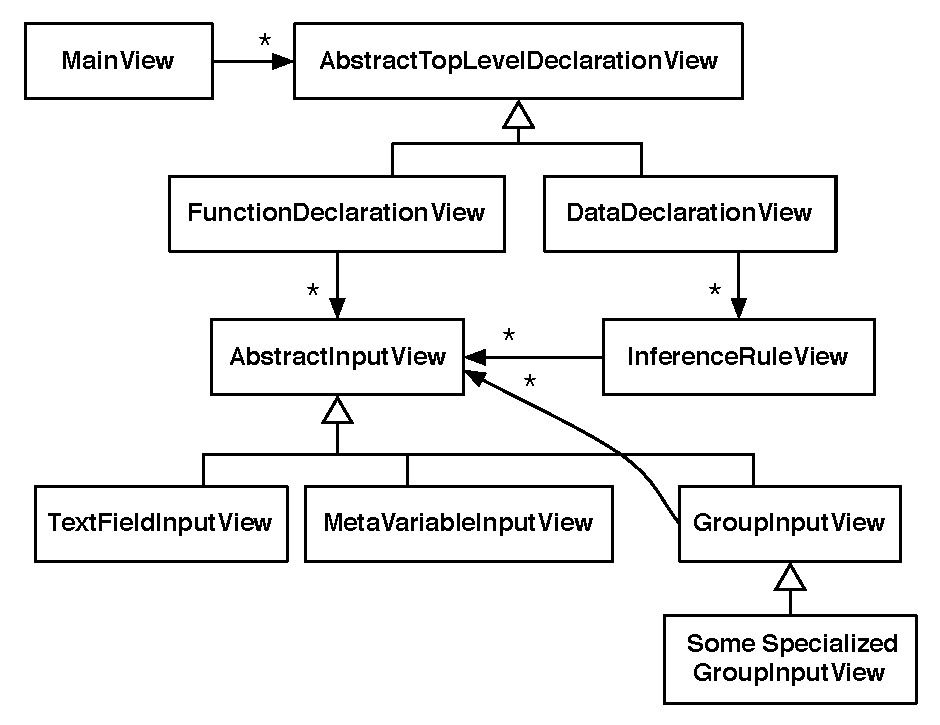
\includegraphics[width=110mm]{diagrams/client_side_class_diagram.pdf}
	\caption{A subset of the client-side diagram showing how the view hierarchy
	almost mirrors the Abstract Syntax tree.}
\label{fig:clientViewArchitecture}
\end{figure}











